\documentclass[10pt,oneside,swedish]{lips}
\usepackage{float}
%\usepackage[square]{natbib}\bibliographystyle{plainnat}\setcitestyle{numbers}
%\usepackage[round]{natbib}

\bibliographystyle{IEEEtran}
\setcounter{tocdepth}{4}
% Configure the document
\title{Teknisk dokumentation}
\author{Projektgrupp 13}
\date{14 december 2022}
\version{1.0}

\reviewed{Zackarias Wadströmer}{2022-12-14}
\approved{}{2022-12-14} %Approved ska vara Anders efter han har gett ett OK att 1.0 kan fastställas.

\begin{document}
\projecttitle{Taxibil-robot}

\groupname{Projektgrupp 13}
\groupemail{TSEA29_2022HT_E7-Grupp13@groups.liu.se}
\groupwww{https://gitlab.liu.se/da-proj/microcomputer-project-laboratory-d/2022/g13}

\coursecode{TSEA29}
\coursename{Konstruktion med mikrodatorer}

\orderer{Anders Nilsson, ISY, Linköpings universitet}
\ordererphone{013-28 26 35}
\ordereremail{anders.p.nilsson@liu.se}

\customer{Anders Nilsson, ISY, Linköpings universitet}
\customerphone{013-28 26 35}
\customeremail{anders.p.nilsson@liu.se}

\courseresponsible{Anders Nilsson, ISY, Linköpings universitetn}
\courseresponsiblephone{013-28 26 35}
\courseresponsibleemail{anders.p.nilsson@liu.se}

\supervisor{Peter Johansson}
\supervisorphone{013-28 1345}
\supervisoremail{peter.a.johansson@liu.se}

\smalllogo{../Figures/LiU_primary_black} % Page header logo, filename
\biglogo{../Figures/logo} % Front page logo, filename

\cfoot{\thepage}
\begin{document}
\maketitle

\cleardoublepage
\makeprojectid

\begin{center}
  \Large Projektdeltagare
\end{center}
\begin{center}
  \begin{tabular}{|l|l|l|l|}
    \hline
    \textbf{Namn} & \textbf{Ansvar} & \textbf{Telefon} & \textbf{E-post}\\
    \hline
    Linus Thorsell & Projektledare & 0765612171 & linth181@student.liu.se\\
    \hline
    Oscar Sandell & Testansvarig & 0709416866 & oscsa604@student.liu.se\\
    \hline
    Hannes Nöranger & Utvecklare & 0733118779 & hanno696@student.liu.se\\
    \hline
    Johan Klasén & Dokumentansvarig & 0730982555 & johkl473@student.liu.se\\
    \hline
    Zackarias Wadströmer & Utvecklare & 0706142029 & zacwa923@student.liu.se\\
    \hline
    Thomas Pilotti Wiger & Konstruktionsansvarig & 0761708593 & thopi836@student.liu.se\\
    \hline
  \end{tabular}
\end{center}


\cleardoublepage
\tableofcontents{}

\cleardoublepage
\section*{Dokumenthistorik}
\begin{tabular}{p{.06\textwidth}|p{.1\textwidth}|p{.45\textwidth}|p{.13\textwidth}|p{.13\textwidth}} 
  \multicolumn{1}{c}{\bfseries Version} & 
  \multicolumn{1}{|c}{\bfseries Datum} & 
  \multicolumn{1}{|c}{\bfseries Utförda förändringar} & 
  \multicolumn{1}{|c}{\bfseries Utförda av} & 
  \multicolumn{1}{|c}{\bfseries Granskad}\\
  \hline
  \hline
  1.0 & 2022-12-14 & Första versionen & Grupp13 & Johan Klasén   \\
  \hline
\end{tabular}

\cleardoublepage
\pagenumbering{arabic}\cfoot{\thepage}

\section{Inledning}
Projektet gick ut på att projektgruppen skulle utveckla en taxibil som uppfyller ett flertal krav vilka förhandlades fram emellan kunden och projektgruppen. Dessa krav finns listade i dokumentet ''Kravspecifikation'' \cite{kravspec}.

\subsection{Den färdiga produkten}
Projektets produkt är en bil som klarar av att köra autonomt igenom ett vägnät. Bilen ska agera taxi, där den hämtar upp en passagerare vid ett stopp och lämnar av dem vid ett annat. Den använder en extern applikation för att ta in styrparametrar och köruppdrag, vilket den använder för att räkna ut hur den ska navigera igenom vägnätet. Bilen är utrustad med sensorer så som kamera och avståndsmätare för att kunna läsa av sin omgivning och köra säkert på vägen.

\begin{figure}[H]%[htbp]
  \centering
  \includegraphics[width=.6\textwidth]{../Figures/Car_Right.jpg}
  \caption{Bild på den färdiga produkten.}
  \label{fig:system-overview}
\end{figure}

\pagebreak

\section{Teori}
Systemet utnyttjar ett flertal kända metoder inom bildbehanling för att kunna navigera sig igenom vägnätet via ett kameraflöde. Merparten av dessa är implementerade med hjälp av externa ramverk som till exempel \emph{''OpenCV''}. Teorin för metoderna som implementeras beskrivs här.

% Preprocessing och/eller Sobel edge och/eller Gaussian Blur?

\subsection{''Sobel operator'' och ''Gaussian blur''}
För att bearbeta bilder i systemet används ''Sobel operator'' och ''Gaussian blur'' vilket båda utnyttjar filter som ändrar färgen av varje enskild pixel i en bild. De applicerar en matris som kallas för filter och lägger den över varje pixel i bilden för att avgöra dess värde. En pixelns färg blir då en viktning av närliggande pixlar där varje medräknad pixels vikt bestäms av filtret. Genom att välja olika matriser kan olika effekter uppnås och är huvudsakliga metoden för att applicera ''Sobel operator'' som hittar kanter och ''Gaussian blur'' som smetar ut bilden.
För att minska fördröjningen för systemet implementeras dessa genom \emph{''OpenCV''} som redan har skapat en snabb och fungerande lösning av dessa.

\subsection{Sliding windows}
I datorseendet krävs det att kantlinjernas bana hittas. De pixlar i bilden som representerar någon kant fås från tidigare steg men för dela upp dem för respektive väglinje implementeras \emph{''Sliding windows''}. Denna teknik är simpel och skapar tillräckligt bra fördelningar vilket är lämpligt för systemet då det inte klarar av särskilt tunga processer. Den hittar pixlar tillhörande en linje så den används en gång per vägkant. \\

\noindent
''Sliding windows'' tar en två dimensionell matris fylld av intressanta värden och andra värden, i systemet representerade av ettor respektive nollor. Först hittas den troligaste starten av en linje genom att kolla vilken kolumn som har störst förekomst av ettor, denna kolumn utgör procedurens startpunkt. För vägkanterna hittas första vägkantens startposition genom att inspektera bildens vänstra halva och den andra vägkantens startposition genom den högra halvan. \\

\noindent
Sedan startar proceduren med att hitta alla punkter med ettor i ett fönster mitt mitten på den kolumnen. Alla dessa punkter läggs till punkter för vägkanten och av dem i fönstret räknas en medelposition ut varav dess kolumn används för att placera mitten av nästa fönster som placeras precis över det aktiva fönstret. I det nya fönstret repeteras processen tills bildens topp har nåtts. \\

\noindent
Om man ritar upp fönstrena ser det ut som att dem glider på varandra och på så vis inkapslar alla intressanta pixlar för vägkanten, därav namnet ''Sliding windows''.

\pagebreak

\section{Systemet}
\label{sec:systemet}
Bilen är uppbyggd utav tre separata moduler som samverkar genom att skicka data mellan varandra. En av modulerna, \emph{Kommunikationsmodulen}, skickar även data till och tar emot data ifrån den externa applikationen som tillåter en användare att styra bilens beteende. De andra två modulerna \emph{Styrmodulen} och \emph{}{Sensormodulen} består av två \emp{AVR} mikroprocessorer av varianten ATmega 1284p. \\
Sensormodulen ansvarar för att samla in data från de externa sensorer som används och styrmodulen ansvarar för bilens framdrivning genom att styra bilens styrservo och drivmotor.
Data från sensormodulen som ska till styrmodulen skickas igenom kommunikationsmodulen och därav utgör kommunikationsmodulen bilens centrum.

\begin{figure}[H]%[htbp]
  \centering
  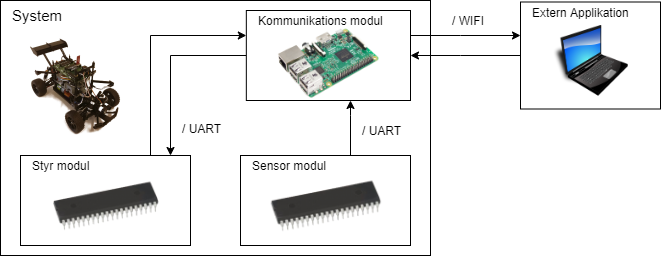
\includegraphics[width=.7\textwidth]{../Figures/tekdok-overview.png}
  \caption{Övergripande blockschema på systemet.}
  \label{fig:system-overview}
\end{figure}


De olika delarna i systemet kommunicerar med varandra genom att skicka data över UART. Datan som skickas över UART följer ett specificerat format som beskrivs i Tabell \ref{table:format}. 
\begin{table}[h!]
\centering

 \begin{tabular}{||c c c c c||} 
 \hline
 Commando & Label & Content & Target & Source\\ [0.5ex] 
 \hline\hline
 keypresses & kp: & f=<0/1>:l=<0/1>:b=<0/1>:r=<0/1>: & Control Module & App \\ 
 emergencystop & es: & stop if label received & Control Module & ALL \\
 debugpid & db: & esp=<int>:sp=<int>:est=<int>:st=<int>: & App & Control Module\\
 switchmode & sm: & m=<auto(0)/manual(1)>: & Control Module & App\\
 speed sendpid & spp: & p=<int>:i=<int>:d=<int>: & Control Module & App \\
 steering sendpid & stp: & p=<int>:i=<int>:d=<int>: & Control Module & App\\
 error & er: & st=<int>:sp=<int>: & Control Module & OpenCV\\
 telemetry & tm: & s=<int>:d=<int>: & Control Module & Sensor\\
 mission & mi: & s=<ascii>:p=<ascii>:e=<ascii>: & OpenCV & App\\
  Toggle Detection & td: & d=<int>:& Control Module & App\\[1ex] 
 \hline
 \end{tabular}
\caption{Formatet av textsträngarna som skickas mellan de olika modulerna}
\label{table:format}
\end{table}

\pagebreak
\section{Modulerna}
\label{sec:modulerna}
Alla moduler i systemet är utbytbara så att en modul som uppfyller samma kommunikations protokoll kan ersätta en modul i systemet. Nedan följer en beskrivning av modulernas olika delar och funktionalitet.

\subsection{Kommunikationsmodul}
Pågrund av valet av hårdvara utgör kommunikationsmodulen centrum för mycket av systemets funktionalitet.

\subsubsection{Hårdvara}
Kommunikationsmodulens hårdvara består av en processorkärna på en Raspberry Pi 3b. Detta ger den tillräckligt med prestanda för att kunna agera kommunikationsserver mellan alla moduler, även till den externa applikationen som kommunicerar över wifi. Då raspberry pi:n kan kopplas direkt till kameran och kan klara av mera arbete ansvarar den även för datorseendet.

\subsubsection{Start Taxi Script}
Detta är ett python script som startar alla system som körs på kommunikationsmodulens mikrodator.
Detta script startas vid startup via en Systemd Daemon, som även agerar förälder till alla underprocesser som skapas.
Efter alla processer startats dödas scriptet.
Scriptet ansvarar även för att identifiera vilken modul som har vilken UART-port via ett simpelt handskak.
AVR skickar vad den är, exempelvis \emph{''Communication-Module''} via UART och scritpet skickar tillbaka \emph{''ACK;''} och sparar vilken modul det var som var kopplad på den UART porten. Sedan startas alla följande script som körs på kommunikationsmodulen: Server Script, AVR Kommunikation (på båda UART portarna) och Datorseende / Pathfinding scripten.

\begin{figure}[htbp]
  \centering
  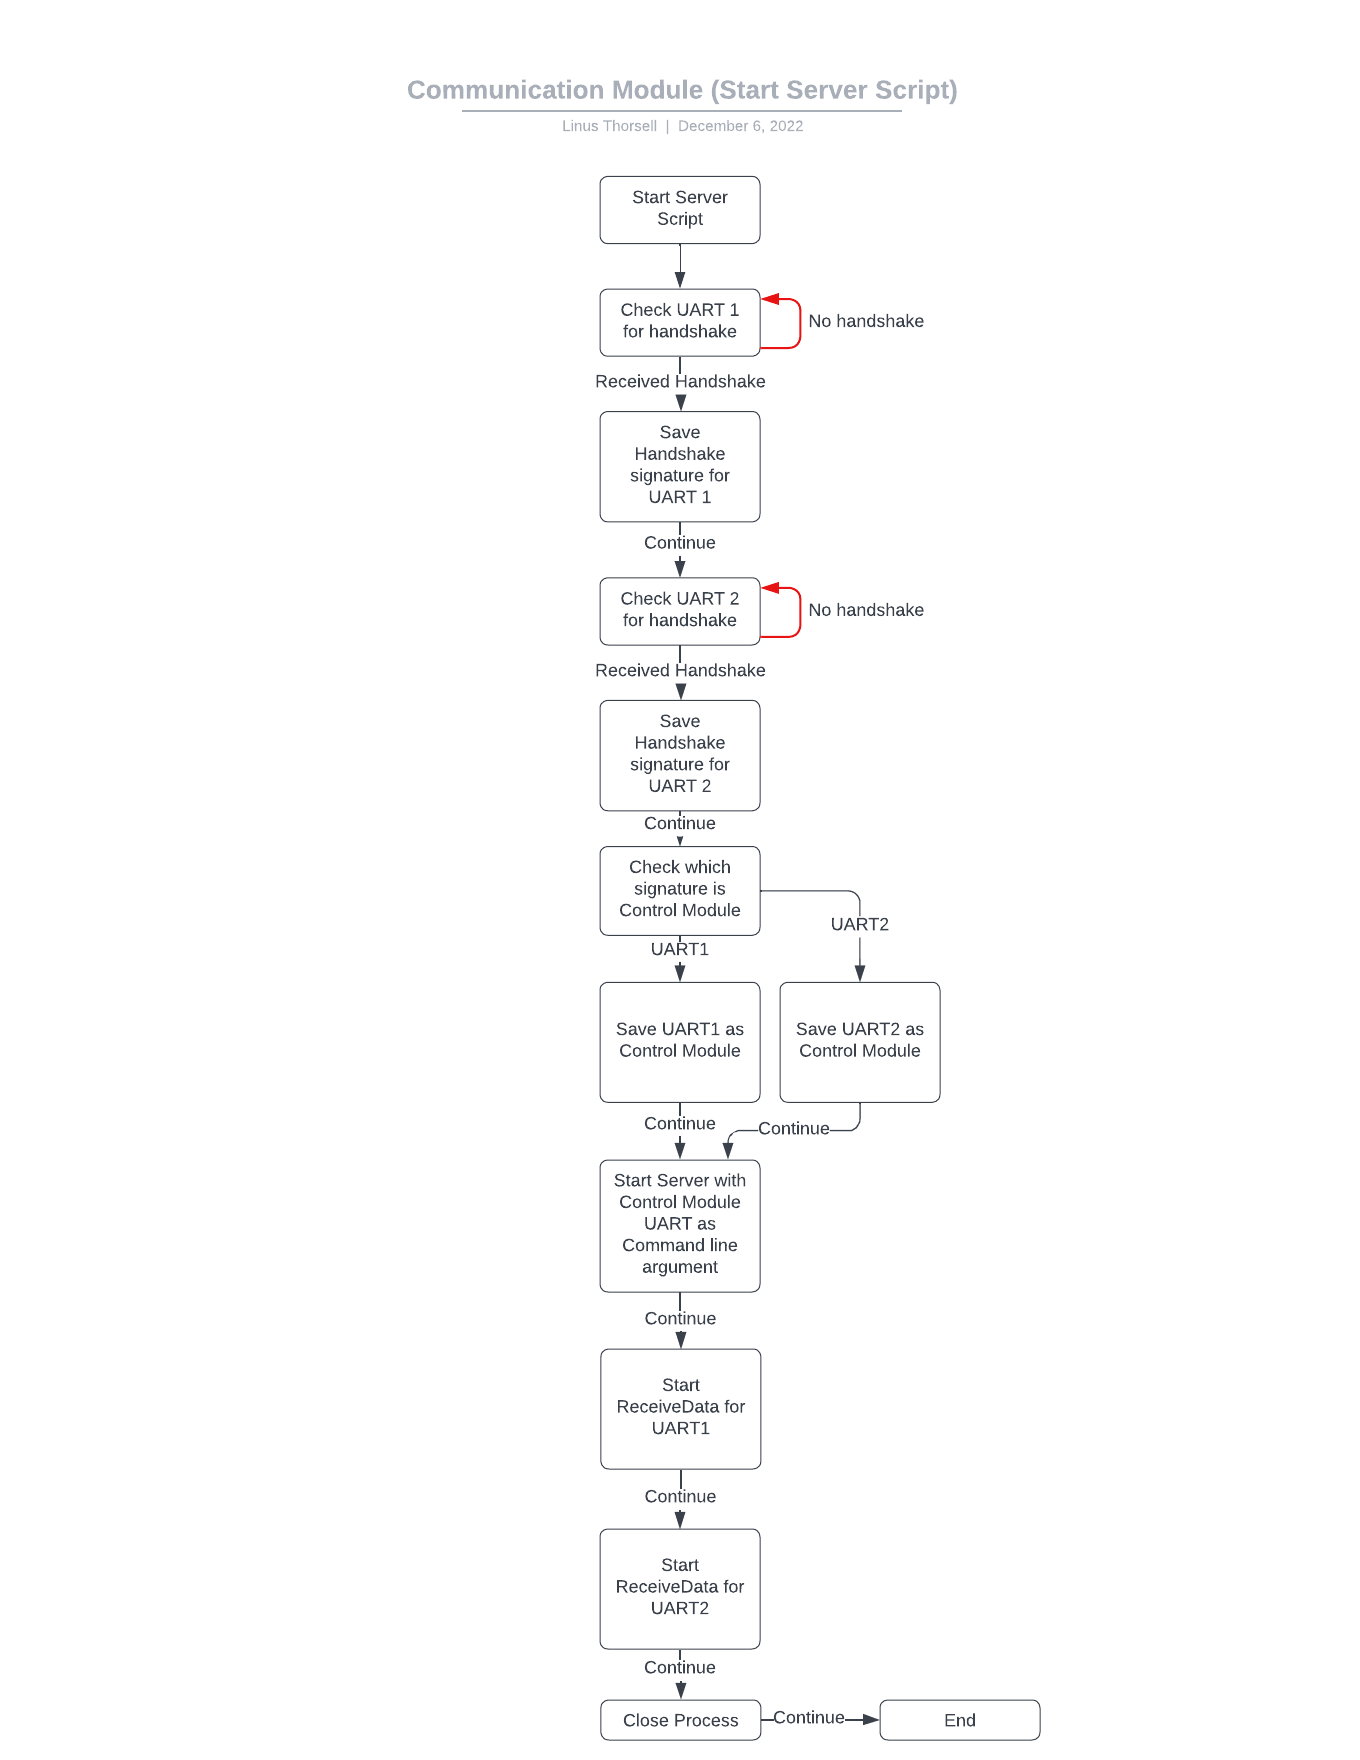
\includegraphics[width=0.7\textwidth]{./Figures/CM_Start_Server_Script.png}
  \caption{Blockschema för kommunikationsmodulens startscript.}
  \label{fig:CM_Start_Server_Script.png}
\end{figure}

\subsubsection{Server Script}
Detta Python script är huvudscriptet som hanterar all kommunikation mellan Sensor-, Styr-, och Kommunikationsmodul samt WebApp, och ett blockschema för programmet kan ses i Figur \ref{fig:CM_Server_Script.png}.
Det startas med ett kommandradsargument som är vilken UART port som kontrolmodulen är kopplad till.
Varje gång servern får in-data via UART eller via en Socket så kollar den vilket label som sitter i början av strängen och skickar endast datan till de som faktiskt behöver använda den. Ett exempel på detta är att resterande kommunikationsmodul inte behöver få emergencystop kommandot, så det skickas bara till kontroll modulen.

\begin{figure}[htbp]
  \centering
  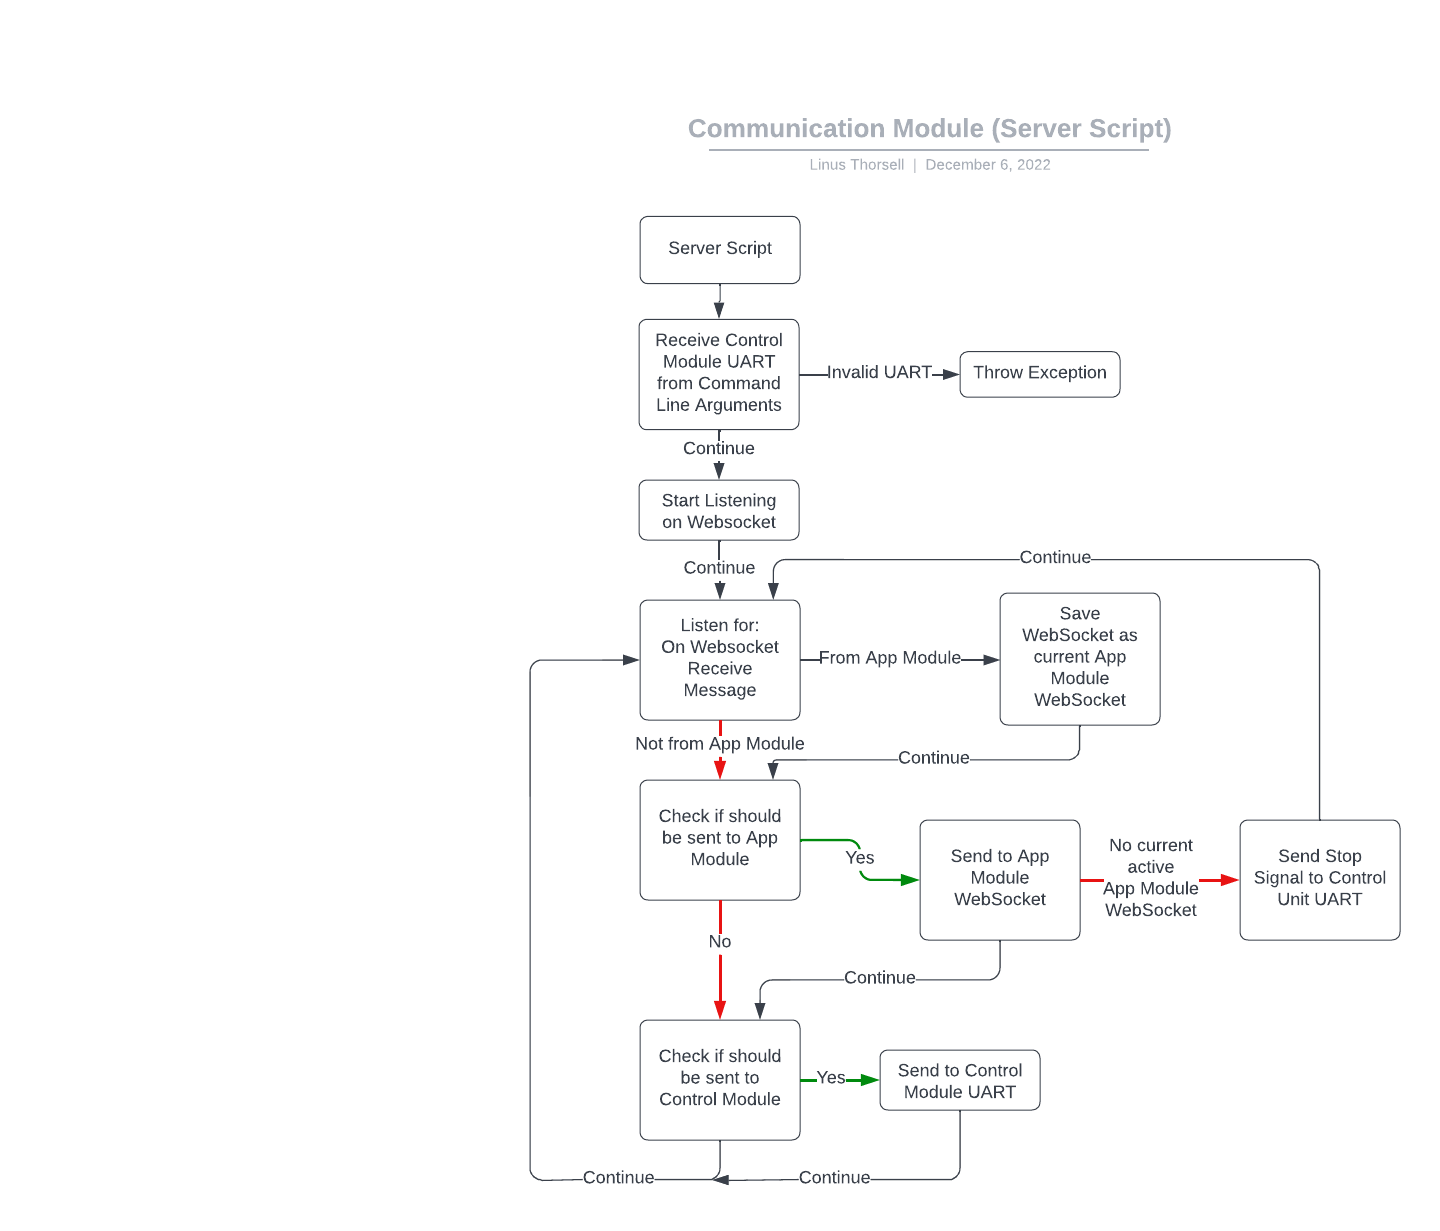
\includegraphics[width=0.7\textwidth]{./Figures/CM_Server_Script.png}
  \caption{Blockschema för kommunikationsmodulens server.}
  \label{fig:CM_Server_Script.png}
\end{figure}

\subsubsection{AVR Kommunikation}
Kommunikationen mellan kommunikationsmodulen och sensor- respektive styrmodulen körs via ett Python script. Scriptet öppnar en UART kommunikation med den andra modulen och skickar all relevant data dit den ska, till exempel vidare till Servern via en Socket. Ett blockschema för förloppet finns i Figur \ref{fig:CM_Receive_Data_Script.png}.

\begin{figure}[htbp]
  \centering
  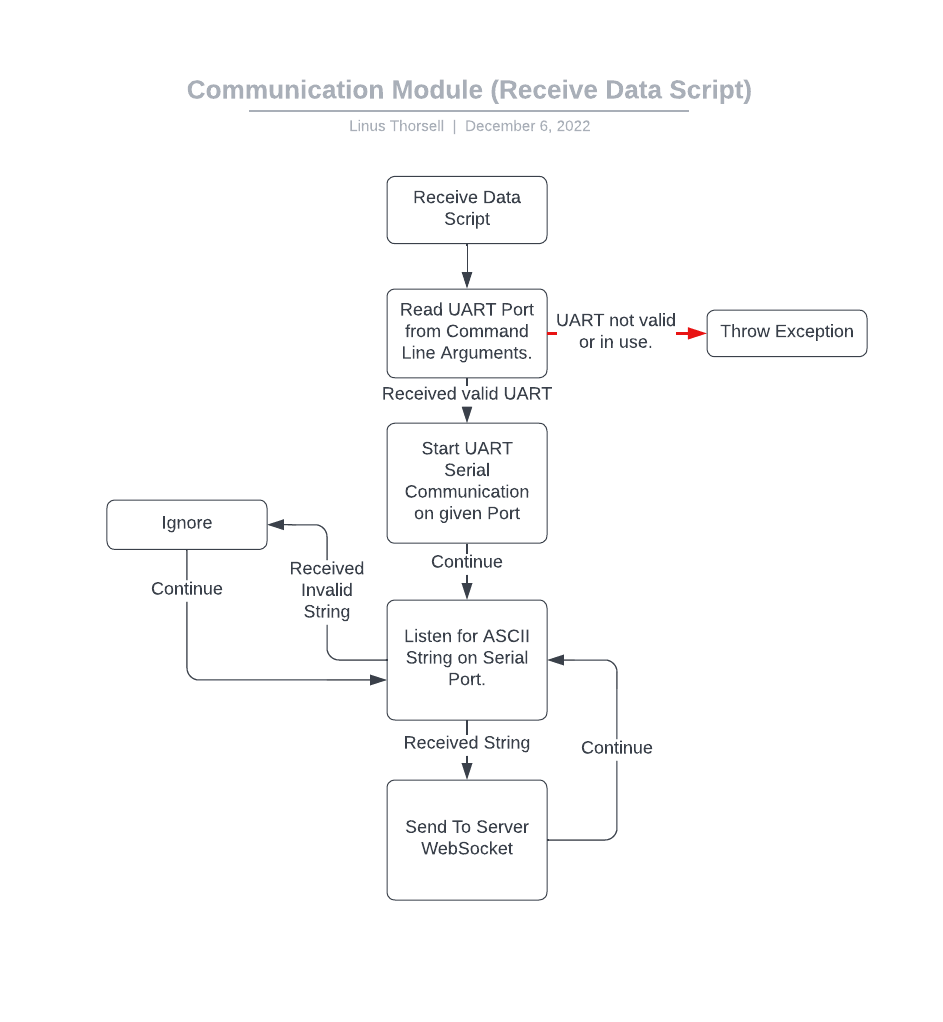
\includegraphics[width=0.7\textwidth]{./Figures/CM_Receive_Data_Script.png}
  \caption{Blockschema för kommunikationsmodulens AVR kommunikationsscript.}
  \label{fig:CM_Receive_Data_Script.png}
\end{figure}

\subsubsection{Pathfinder}
Pathfindern är till för att hitta den kortaste vägen från startplatsen till upphämtningsplatsen och sedan från upphämtningsplatsen till avlämningsplatsen. Pathfindern skrevs i programmeringsspråket python och kan lätt anropas från huvudprogrammet.

\subsubsection{Grafen och Algoritmen}

För att lösa problemet med att få fram den kortaste vägen i grafen används en uppsättning noder, där varje plats i banan (Station A, B, C, D, E, F, Kors 1 och Kors 2) representeras av två noder och en uppritad variant av grafen kan ses i Figur \ref{fig:Grafen_noderna.png}. Varje nod representerar en position och en körriktning då vi vill kunna vara på samma fysiska plats två gånger per körrunda, detta då bilen skulle kunna vända om och köra tillbaka genom punkten för att komma fram med rätt sida vänd mot målet. \\

\begin{figure}[H]
  \centering
  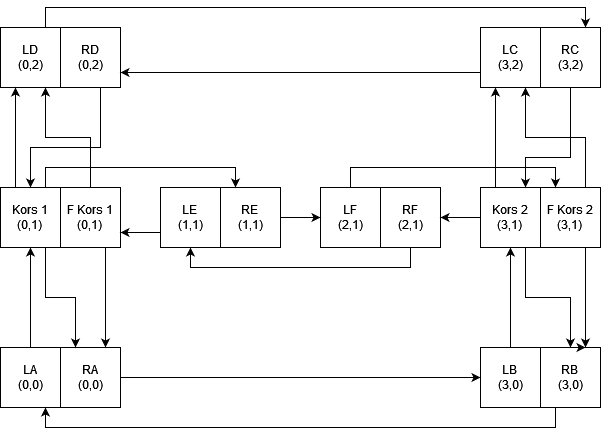
\includegraphics[width=1\textwidth]{./Figures/Grafen_noderna.png}
  \caption{Grafen som används i Pathfindern.}
  \label{fig:Grafen_noderna.png}
\end{figure}

\noindent
När det kommer till självaste pathfinding-algoritmen används en DFS som söker fram alla vägar som når till målet, för att sedan välja den väg som är kortast. Om två vägar är lika långa så väljs den väg som går igenom ''E'' och ''F'' vilket garanterar den kortaste vägen i denna graf. Anledningen till att DFS valdes var för att vi ville ha en rekursiv funktion då det kändes lättare att få fram ett bra resultat. Anledningen till detta var för att vi behövde ett extra kondition i if statementet i DFS när man ska utforska alla noder. I en normal DFS algoritmen så utforskar man bara noden om den noden man ska utforska inte har utforskats tidigare, i detta fall vill vi lägga till ett fall som är att vi utforskar noden om den noden vi vill utforska inte ligger på samma plats som den tidigare noden vilket då eliminerar problemet att bilen skulle vilja vända om 180$^{\circ}$. Programflödet av Pathfindern syns i Figur \ref{fig:Grafen_noderna.png}:

\begin{figure}[htbp]
  \centering
  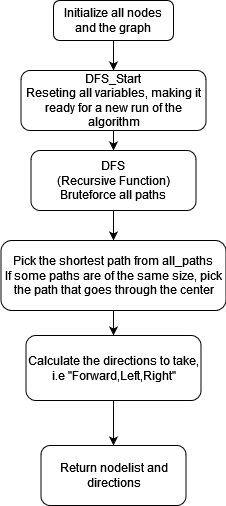
\includegraphics[width=0.35\textwidth]{./Figures/Pathfinder.png}
  \caption{Ett simpelt programflöde över Pathfindern.}
  \label{fig:Grafen_noderna.png}
\end{figure}

\clearpage

\subsection{Sensormodul}
Sensormodulen består av en ATmega 1284P och dess uppgift är att samla och bearbeta den data som bilen genererar när den åker, d.v.s. hastighet via en odometer med hallsensorer och detektion av eventuella föremål framför bilen som detekteras med hjälp av en ultraljudsensor.
Datan skickas vidare i jämna intervaller till kommunikationsmodulen via UART som sammanställer den med data från övriga moduler och för den vidare till styrmodulen och webb-applikationen. 


\subsubsection{Odometer}

Bilen är utrustad med två halleffektsensorer monterade i anslutning till bakhjulen. På bakhjulen sitter tio magneter placerade med jämnt mellanrum och med hjälp av dessa kan en hastighet mätas upp. När ett tillräckligt starkt magnetfält passerar hallsensorn ger den utslag och ger en hög utsignal. Signalen är kopplad till en extern avbrotts-pin (INT1) på AVR:en. Tillhörande avbrottsrutin är sedan inställd att köras på varje stigande flank på signalen och ökar varje gång en räknare som håller koll på hur många gånger (antal ''tick'') en magnet har passerat sensorn under ett visst intervall.
Detta används sedan för att räkna ut hastigheten som frekvensen av magneter per tidsintervall.

\subsubsection{Ultraljudsensor}
Ultraljudsensorn består av en SRF04 och fungerar genom att skicka ut ekopulser som kan studsa på eventuella föremål framför sensorn och sedan mäta tiden det tar för ekot att studsa tillbaka för att på så sätt avgöra avstånd till föremålet. \\ %referens till SRF04
\noindent
Sensorn styrs med signalen \emph{Trigger Input} och tid fås via signalen \emph{Echo Pulse Output} och timingen kan studeras närmre i Figur \ref{fig:us-timing}. En mätning startas via att en 10 μs lång puls skickas till \emph{Trigger Input} för att signalera starten på en mätning. En kort tid därefter skickar ultraljudsensorn ut eko-pulserna och drar \emph{Echo Pulse Output} hög för att visa att den har börjat lyssna på studset av ekot. När ekot når tillbaka (eller man når en timeout på 36 ms) dras \emph{Echo Pulse Output} låg igen och bredden på pulsen som skickas motsvarar alltså avståndet till föremålet. För att underlätta implementeringen mäts dock den totala tiden räknat från den fallande flanken på startpulsen fram tills fallande flank på \emp{Echo Pulse Output}. \\

\noindent
Detta hanteras via AVR:en genom att koppla \emph{Trigger Input} till en pin länkat till en intern timer (OC0A) och \emph{Echo Pulse Output} till en extern avbrotts pin (INT2). Timer0 har ställts in så att den skickar hög output i 10 μs och sedan stänger av sig själv för att hantera startsignalen till \emph{Trigger Input} och sätter en starttid för mätning. Och för \emph{Echo Pulse Output} är INT0 inställt så att man får en interruptrutin på fallande flank för att få en sluttid på mätningen. \\

\noindent
Det uppmätta värdet används sedan helt enkelt som kollisionsdetektion för bilen. Blir den uppmätta tiden tillräckligt låg för att hamna under ett satt gränsvärde vet man att det finns föremål framför bilen och att den behöver stanna, men denna tolkning görs dock i styrmodulen.

\begin{figure}[H]
  \centering
  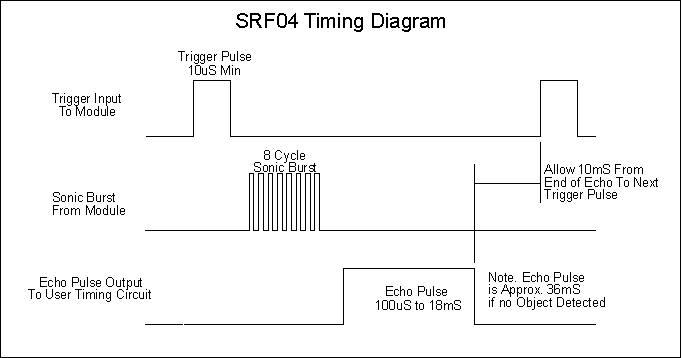
\includegraphics[width=.60\textwidth]{./Figures/srf04timing.png}
  \caption{Tidsdiagram för ultraljudsensorns signaler. \emph{Trigger Input} innebär starten av en mätning där sensorn svarar med att dra \emph{Echo Pulse Output} hög så fort den är redo att lyssna på ett eko och låg igen efter 36 ms (timeout) eller så fort ekot har tagits emot, vilket som kommer först.}
  \label{fig:us-timing}
\end{figure}

\subsubsection{Programkod}

Vid uppstart av modulen körs först en initieringsrutin som konfigurerar och startar bland annat portinställningar, minnesbuffertar, timers och och de fem avbrottsrutinerna. Den första avbrottsrutinen är en timer kopplat till AVR:ens interna räknare Timer1. Den körs en gång i millisekunden från och med start och används för att kolla hur mycket tid som har förflutit och på så sätt räkna ut tillsskillnader. Den ser också till att vid satta tidsintervall starta Timer0 för att aktivera ultraljudssenorns startpuls. En andra avbrottsrutin ansvarar sedan för att stänga av Timer0 och avsluta startpulsen.
Den tredje avbrottsrutinen hanterar mottagning av data från UART och de sista två hör till respektive sensor och har nämnts ovan.\\

\noindent
Huvudprogrammet är inte särskilt stort, den har ett handskak i början som upprepat skickar ''sensor\_module'' till kommunikationsmodulen som sen skickar ett ''ACK'' tillbaka. Därefter hamnar sensormodulen i en inre loop där den i satta tidsintervall beräknar tiden det tar för ljudvågen att färdas fram till ett hinder och sedan tillbaka till sensorn om den har fått färsk data. Loopen beräknar sedan även ut hastigheten och sammanställer all data för att sedan skicka den vidare till kommunikationsmodulen enligt specificerad standard i Tabell \ref{table:format}.

\begin{figure}[H]%[htbp]
  \centering
  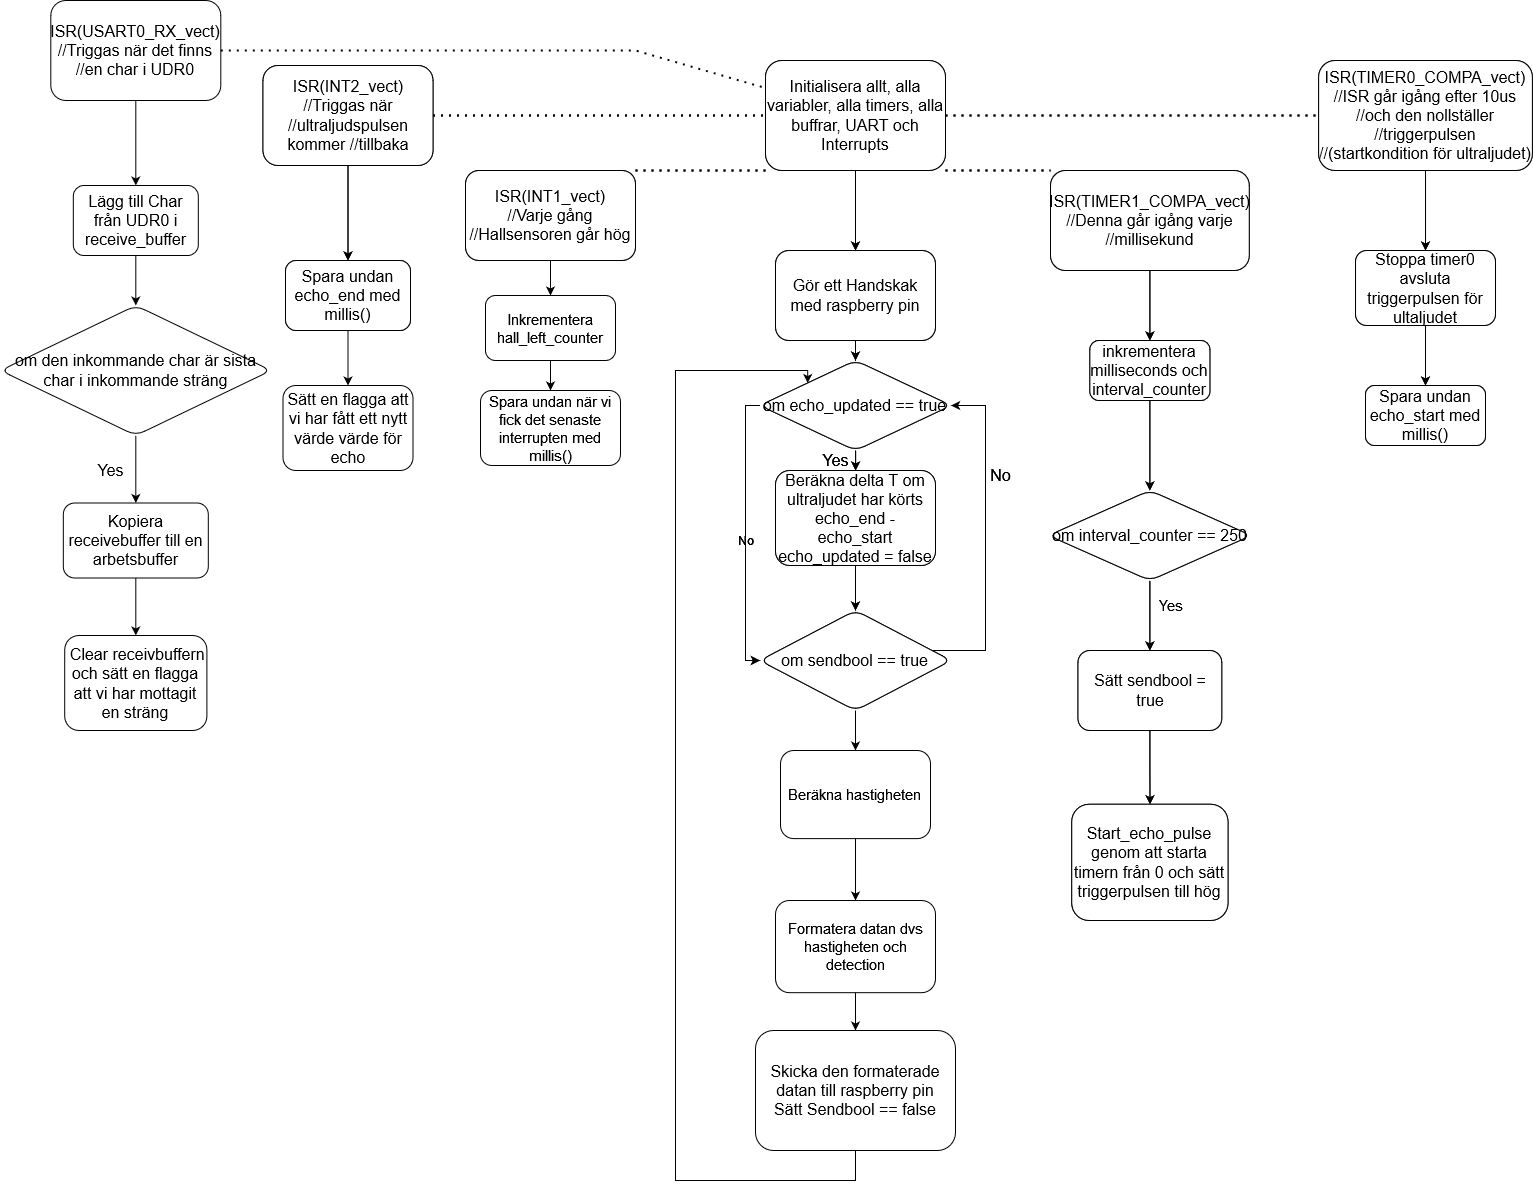
\includegraphics[width=1\textwidth]{./Figures/Sensormodule_blockschema.png}
  \caption{Blockschema över sensormodulen}
  \label{fig:sensor-blockschema}
\end{figure}

\subsection{Styrmodul}
Styrmodulen består av en ATmega 1284P som är kopplad till Raspberry Pin via UART och är även kopplad till bilens motor och styrservo via ett kontaktdon i skelettet. Vi använder oss utav pulsmodulering för att styra motorn och styrservot.

\subsubsection{Pulsmodulering}
Bilens motor och servo styrs pulsmodulering. Detta sker med hjälp av styrmodulens inbyggda timrar och pulsbreddsmodulatorer. Pulserna kommer från Timer1 och Timer3, den ena timern har en periodtid på 0.5 ms och styr motorn medans den andra har en periodtid på 20 ms och styr styrservot. Pulsbredden sätts genom att skriva till registret OCR1A respektive OCR3A. Pulsen som styr motorn kommer från port PB5 och den som styr styrtservot kommer ifrån PB6 kopplade till bilens skelett. 

\subsubsection{Avbrottsrutiner}
Styrmodulen har två avbrott med tillhörande avbrottsrutiner. Den ena avbrottsrutinen är relaterat till UART och tar en char ifrån motagningsregistret UDR0 och sparar charen i en buffer. Avbrottet triggas när det finns data i UDR0 vilket avgörs av RX pinnen blir hög vilket då triggar avbrottet. Den andra avbrottsrutinen är en intern avbrottsrutin och aktiveras varje gång det har gått 1 millisekund och används till att få en fungerande millis() funktion så att vi kan få hur många millisekunder det har gått sedan programmet startades. 

\subsubsection{Mainfunktion}
Styrmodulens huvudprogram består av tre delar, Den första delen av programmet initierar variabler, interrupts och buffertar. Den andra delen är en handskakning där styrmodulen upprepat skickar ''control\_module'' till Raspberry Pin så att den kan avgöra vilken som är Styrmodulen och den tredje delen av mainfunktionen är en whileloop som har hand om allt annat. Det som den sista whileloopen tar hand om är att parsea meddelandet som kom från Pi'n och sedan baserat på detta gör den olika kommandon såsom att köra i olika riktningar, gasa och stoppa.

\subsubsection{Parsern}
Parsern får data i form av en sträng via UART sedan plockar styrmodulen ut den relevanta datan som finns i strängen. Datan är i formetet som syns i tabell \ref{table:format} på sida \pageref{table:format}. Denna data används för allt ifrån till att styra bilen, gasa, få info om eventuella hinder och får även hastigheten.

\subsubsection{Styrning via PID Reglering}
För att hålla sig på vägen vid autonom körning kör styrmodulen en simpel PID loop. Denna körs varje gång modulen får ett nytt fel från kommunikationsmodulen via UART. Det betyder att regleringen körs så ofta den kan på det nya felet.

\subsubsection{Hastighet via PID Reglering}
För att hålla en konstant hastighet under körning så har bilen en PID loop som uppdaterar hastigheten varje gång sensormodulen skickar data till kontroll modulen, detta ger om den tunas för det en mycket mjuk start och mycket mjuk stopp vid upphämtning / avlämningsplatserna.

\begin{figure}[H]
  \centering
  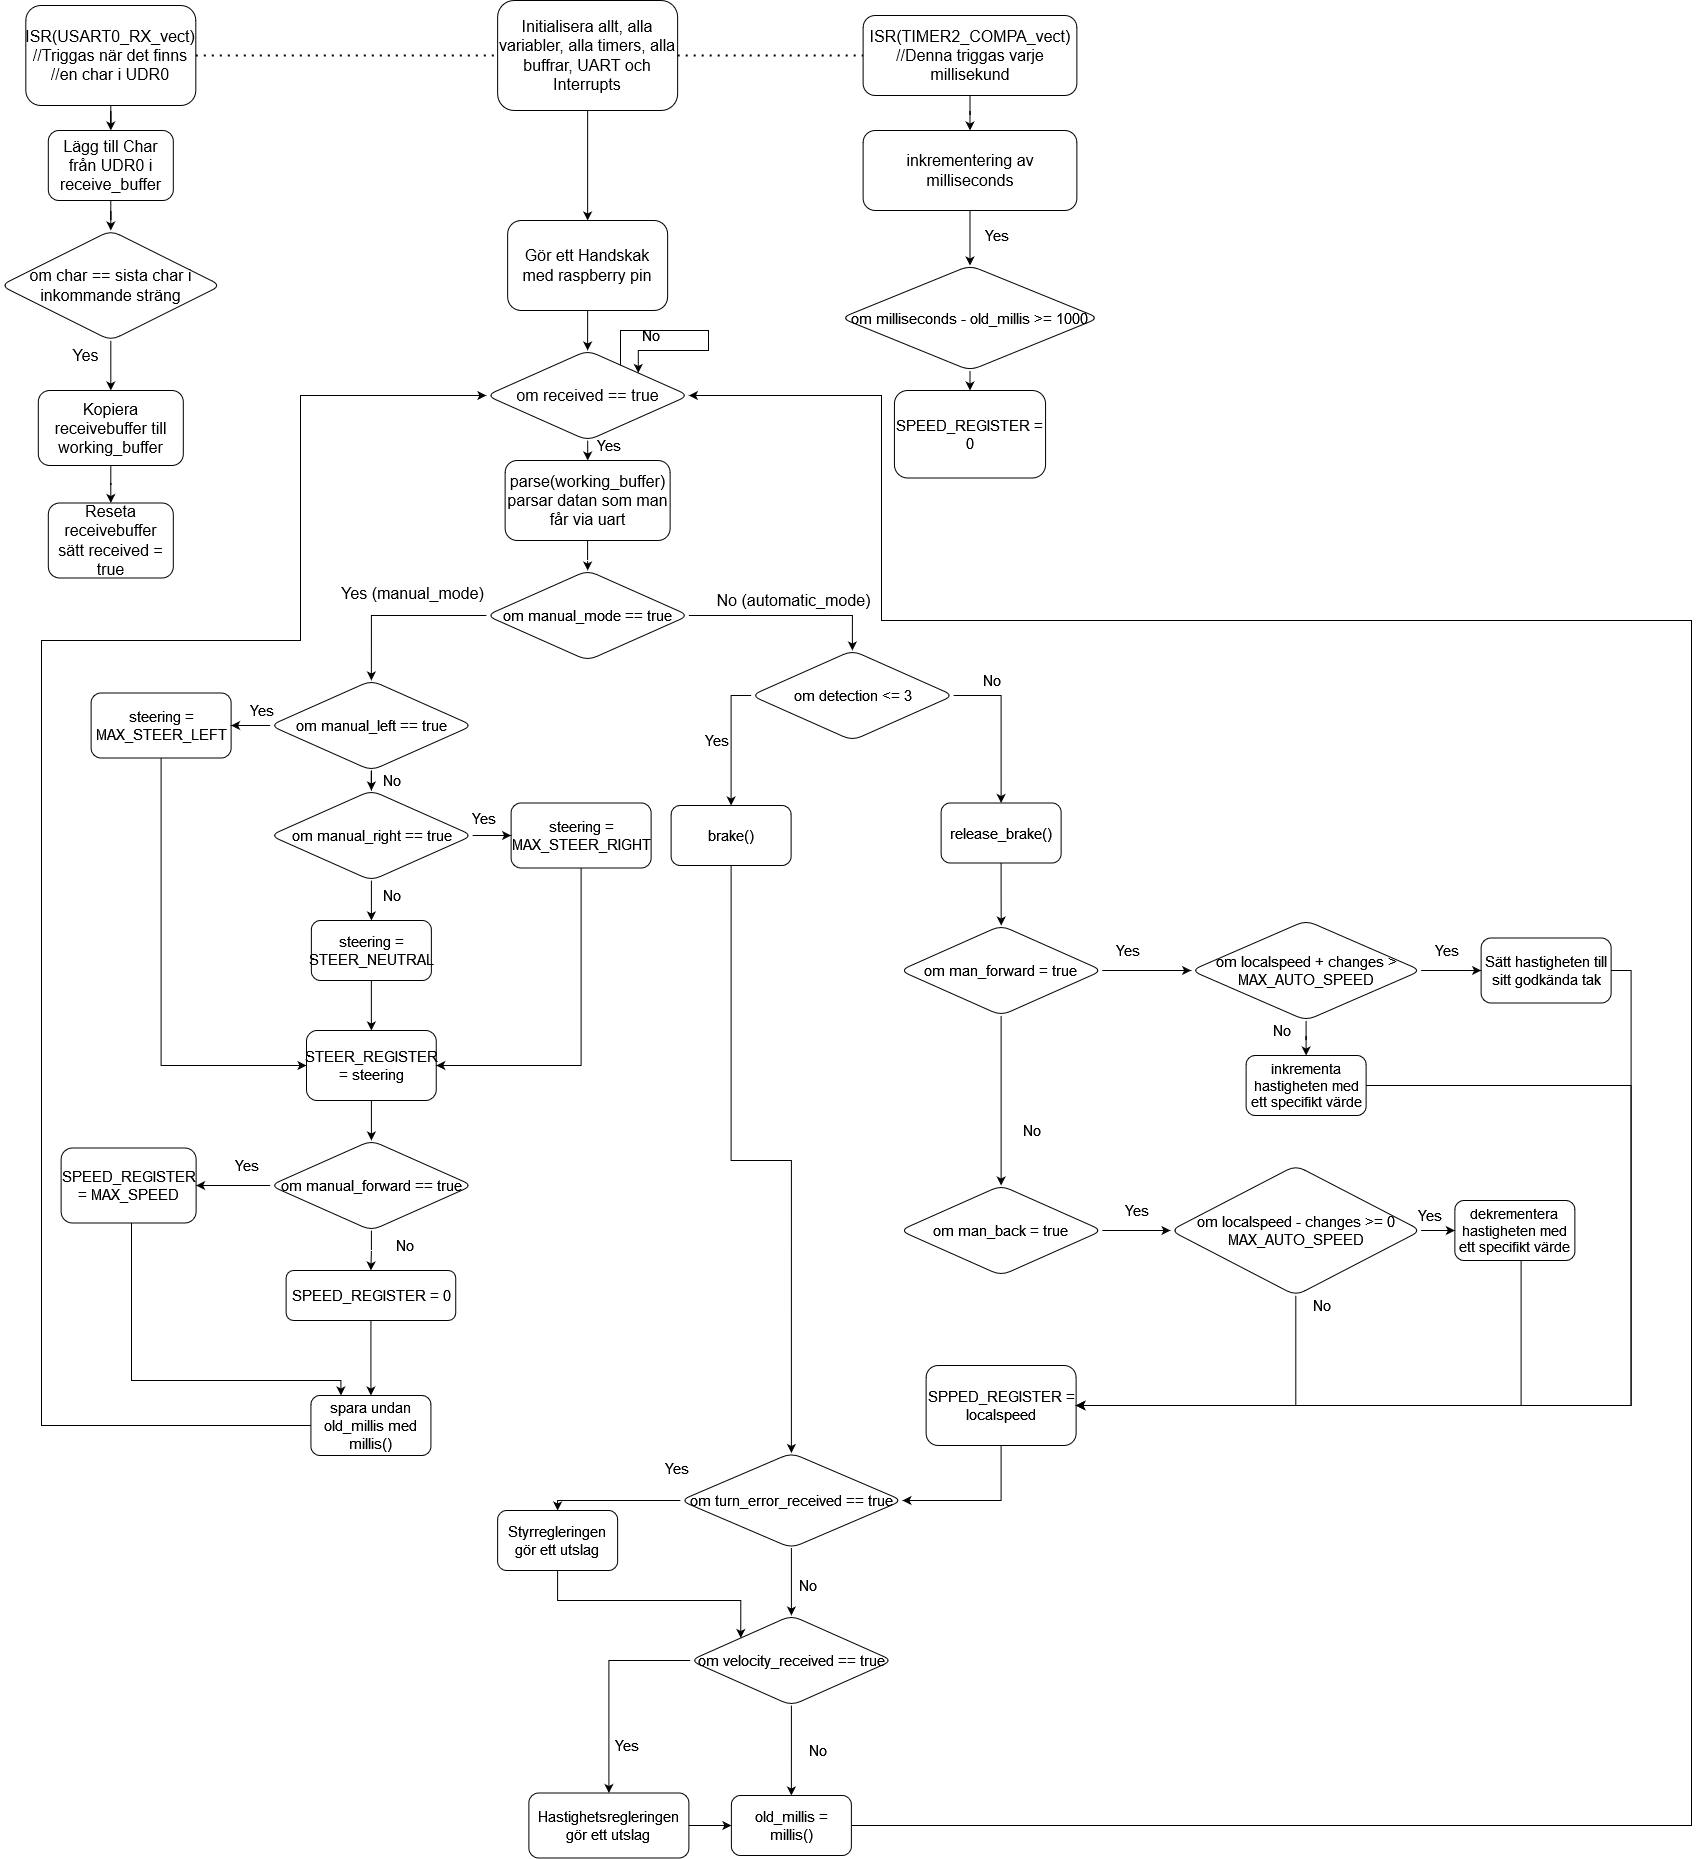
\includegraphics[width=1\textwidth]{./Figures/ControlModule_blockschema.png}
  \caption{Ett detaljerat blockschema över styrmodulen.}
  \label{fig:Grafen_noderna.png}
\end{figure}



\cleardoublepage

\subsection{Datorseende}
För att navigera sig efter vägen använder bilen sig av datorseende i form av ett script där den kontinuerligt tar bilder och bearbetar dem för att producera fel i form av ett numeriskt värde och sedan förse styrmodulen med den. Utöver kontrollerar scriptet parametrar i samarbete med ''pathfindingen'' som berättar hur scriptet ska hantera särskilda sammanhang och om styrmodulen ska stanna. Dessa är i syfte att navigera sig genom vägnätet och särskilt att hantera korsningar korrekt.

\subsubsection{Bildomvandling}
För att tolka bilden börjar scriptet med att omvandla den så att endast relevant information visas upp och på ett relevant sätt. Detta görs i separata steg som representeras av egna funktioner i koden.\\

\begin{figure}[htbp]
  \centering
  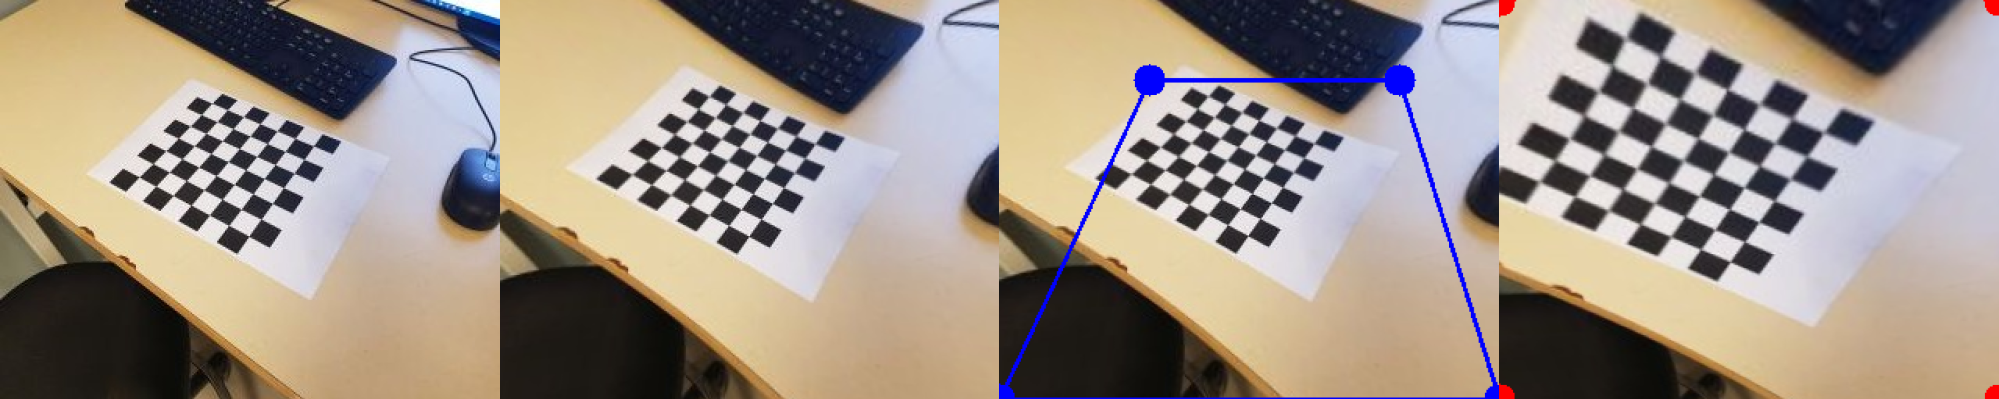
\includegraphics[width=1\textwidth]{./Figures/tekdok-conversion.png}
  \caption{Bildsekvens som visar på omvandlingarna som görs. Första bilden är obehandlad. Andra har tagit bort böjning i linsen. Tredje har 'region of interest' utmarkerats och sista är transformerad för att det området ska täcka skärmen}
  \label{fig:bildomvandling.png}
\end{figure}

\noindent
Först förvrängs bilden för att dess böjning ska försvinna. Denna korrigering är beroende av kamerans lins och dess inställningar och sker genom att omvandla bilden med en förvrängnings matris som beskriver bildens böjning. Då parametrarna för en särskild kamerauppsättning är demsamma räknas dessa ut utanför aktiv exekvering utifrån en uppsättning kalibreringsbilder. Parametrarna sparas sedan undan i en dedikerad fil som sedan hämtas när bilden ska förvrängas under exekvering.\\

\noindent
Näst förvrängs bildens perspektiv. Detta är viktigare för att hantera linjer korrekt och att deras tjocklek samt avstånd från varandra ska representera vägens egenskaper mera korrekt. Detta görs genom \emph{''OpenCV''} som tar koordinater som beskriver det område som ska vridas upp.\\

\noindent
Efteråt hanteras bilden så att kanter markeras ut. Först plockas pixlar med låg färg ut. Dessa representerar vägmarkeringar då dem är svarta och markeras som ettor medan allt annat blir nollor. Sedan används ''Gaussian blur'' för att göra bilden suddig då detta hjälper i nästa steg där alla kanter markeras med hjälp av Sobel operatorn. En suddig bild har jämnare kanter och minskar små störningar som kan framkomma i bilden.\\

\begin{figure}[htbp]
  \centering
  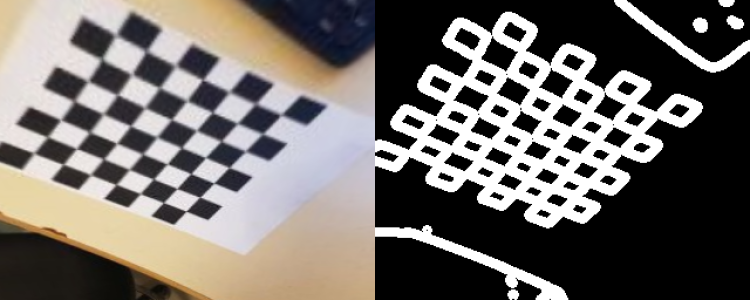
\includegraphics[width=0.5\textwidth]{./Figures/tekdok-edgemarking.png}
  \caption{Bildsekvensen visar konverteringen av en bild. Första bilden är den ingående bilden och den andra är där kanter har markerats.}
  \label{fig:kantmarkering}
\end{figure}

\noindent
Efter all bildomvanlding har bilden omvandlats till en bitmap där ettor utgör vägmarkeringar.

\subsubsection{Tolkning av bild}

Utifrån en bitmap där ettor markerar vägmarkingar utförs olika beräkningar för att producera de styrparametrar som sedan förs till styrmodulen. \\

\begin{figure}[htbp]
  \centering
  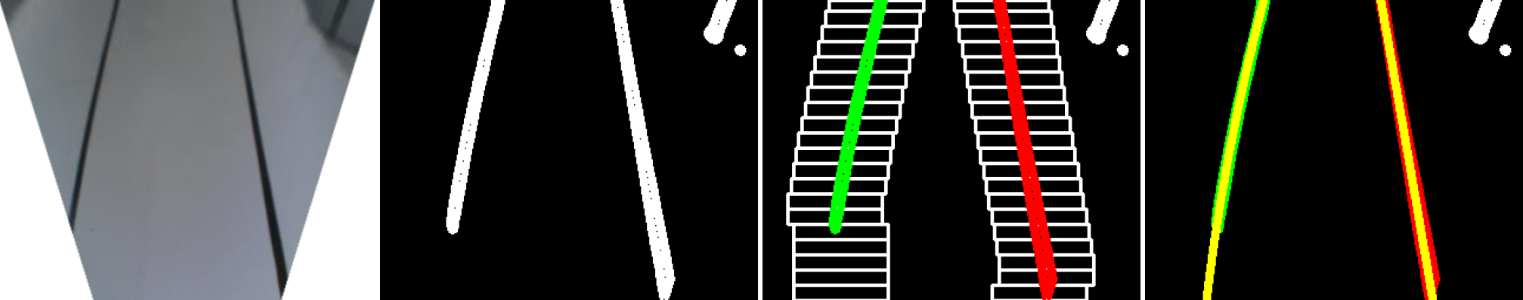
\includegraphics[width=1\textwidth]{./Figures/tekdok-linedetection.png}
  \caption{Bildsekvens som visar på hur en bild tolkas. Första bilden är den bild som ska tolkas efter bildomvandling, som visat i figur \ref{fig:bildomvandling.png}. Det vita området är tillagt för att perspektivet ska bli korrekt men inte kapa bort linjerna. I andra bilden har den omvandlats till en bitmap, som i \ref{fig:kantmarkering}. I tredje används sliding windows för att finna de pixlar som tillhör en av de två vägkanterna som målats i två olika färger. Sista bilden visar linjerna som fås över punkterna för respektive vägkant. }
  \label{fig:bildtolkning.png}
\end{figure}

\noindent
Först markeras positionen av den vänstra och högra väglinjen. Detta görs genom att förekomsten av ettor i varje kolumn markeras ut i ett histogram och sedan får högsta förekomsten i kolumnens första halva markera den vänstra kantens start och högsta förekomsten i den andra halvan för den högra linjens kant.\\

\noindent
Startpunkterna används sedan för att beräkna linjerna i form av andragradskurvor. Detta görs med ''sliding window'' tekniken där förekomsten av punkter inom ett mindre fönster läggs till i punkter för respektive linje och sedan flyttas fönstret upp så att det placeras över det förra fönstret och är centrerad runt förekomsten av punkter i den. Detta repeteras till toppen av skärmen nås. För att finna de två kantlinjerna genomförs processen två gånger om. För varje kantlinje startas processen med att placera första fönstret vid startpunkten för respektive kantlinje, hämtat från tidigare uträkningssteg. Alla punkter för en kantlinje används för att räkna ut en andragradskurva som passar dem så bra som möjligt och representerar vägen.\\

\noindent
Utifrån de två kurvorna räknas två vridgningsfel ut, vilket är hur mycket bilen måste rotera för att träffa banan igen och hur mycket den måste rotera för att ligga parallellt med banan. Eftersom dessa fel ska representera hur bilen ska röra sig framåt förhåller uträkningarna sig till en punkt längre bort på vägen. Exakta avstånd definieras i koden. Felet räknas ut i radianer alltså den exakta vinkeln som bilen måste korrigera.\\

\noindent
Sedan tas de två vridningsfelen för att räkna ut ett enda fel som kan skickas till styrmodulen. Detta fel ska representera hur mycket bilen ska vridas.

\subsection{Styrning från bild}
För att kunna navigera i vägnätet så arbetar datorseendet tillsammans med pathfinding. Från pathfinding får datorseendet information om vilken kant som ska följas i olika skeden i körningen. Under normal körning påverkar båda linjerna bilens styrning men när bilen stöter på en korsning används enbart en. Datorseendet får information om vilken linje som ska följas och kan därmed strunta i den felaktiga linjen och köra åt rätt håll. Vid sväng kan båda linjer hamna utanför kamerans synfält och då ges styrhjälp i form av dödkörning tills dess att linje hittats.

\pagebreak
\section{Slutsatser}

\subsection{Datorseende}
Som datorseendet är utformat just nu måste varje bild gå igenom ett antal processer för att producera styrdata. Dessa har en minimum tid de kan genomföras på för en viss bilduppsättning och efter att ha arbetat med att optimera dem är det klart att denna tidsgräns är ganska stor. \\

\noindent
Det lättaste sättet att minska tiden är genom att minska bildstorleken men det resulterar i förlust av data som förvärrar bilens fel. Detta eftersom linjerna ska passas emot färre punkter och av dessa kommer inte lika många ligga på vägkanten som därav inte kommer väga lika tungt i beräkningarna och kunna resultera i större fel. För att få tillräcklig upplösning men ändå bra tid testades bildens storlek fram men en lämpligare storlek är nog möjligt.

\subsection{PID Reglering}
Med hjälp av datorseendets felvärde kan kontroll modulens PID loopar både hålla bilen i konstant hastighet som bestäms av datorseendet och även reglera styrningen för att hålla sig mitt i vägen.

\subsection{Kommunikation}
Kommunikationen mellan de olika modulerna fungerar bra mellan olika typer av protokoll och överföringstyp, detta på grund av att alla kommandon är baserade på ASCII som alla system på bilen kan förstå. Kommunikationsmodulens huvudserver som använder WebSockets implementerade i Python hanterar all data snabbt och dirigera all data till de mottagarna som skall få denna data.


\clearpage
\bibliography{references}
\clearpage

\appendix
\section{Kopplingsschema}
\begin{figure}[htbp]
  \centering
  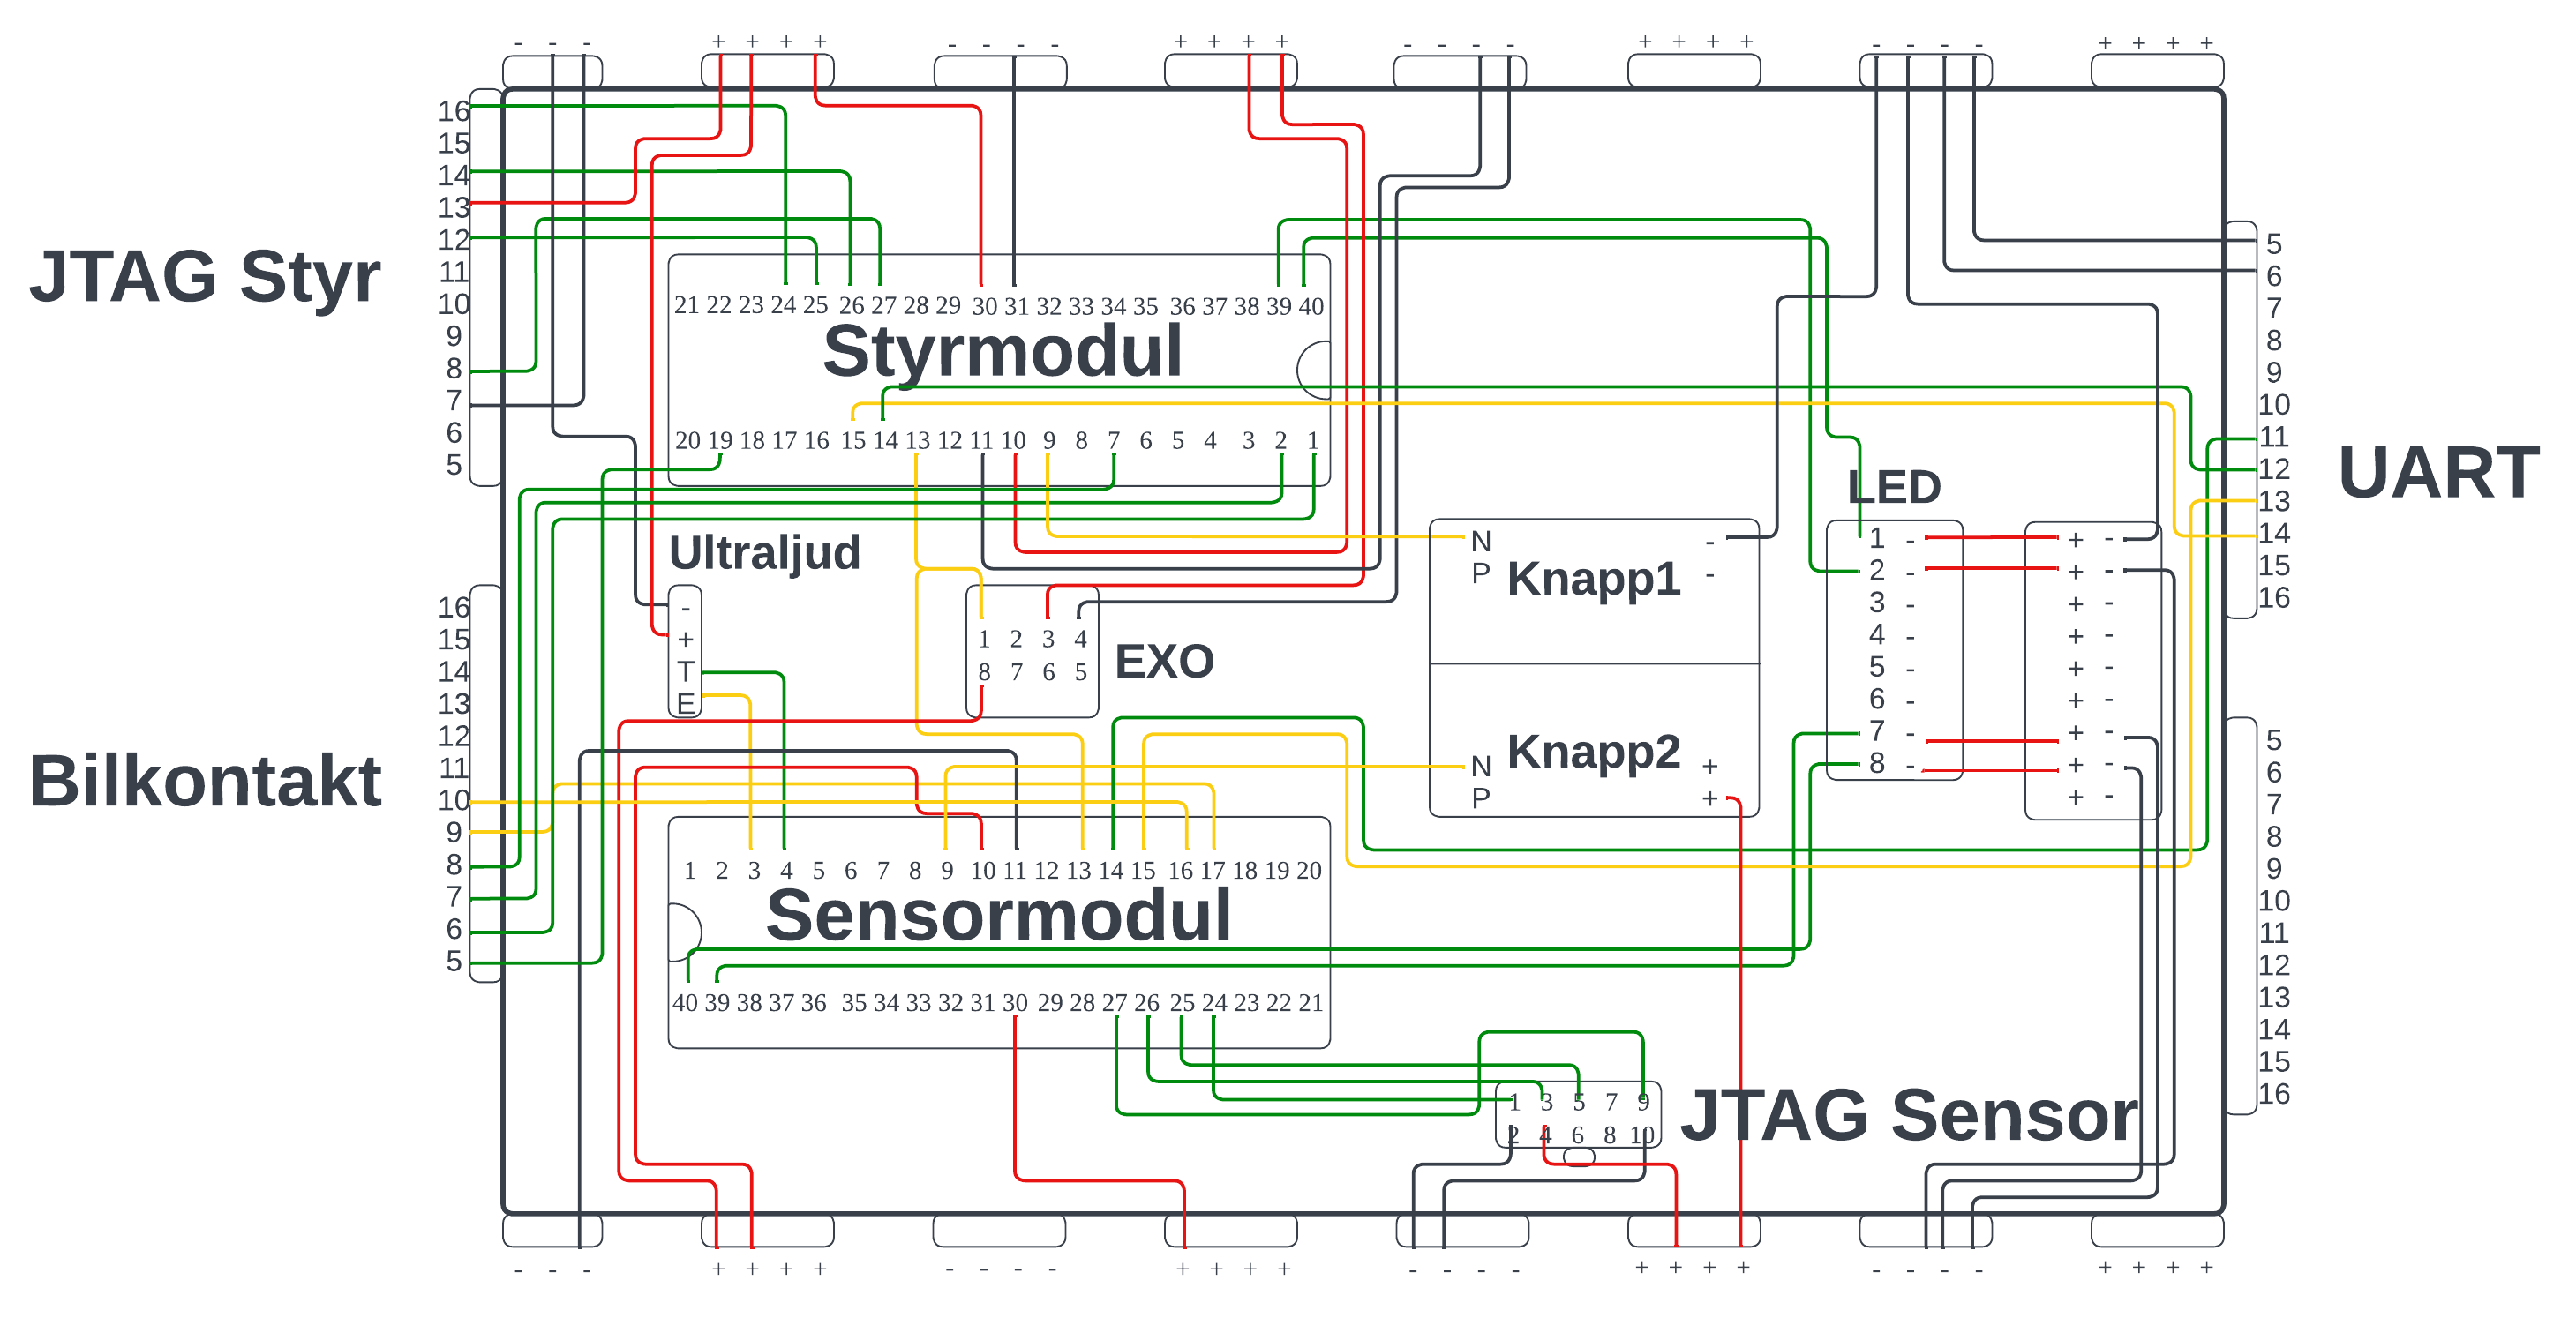
\includegraphics[width=1\textwidth]{Figures/Virning.png}
  \label{fig:virning.png}
\end{figure}

\begin{longtable}{|c|p{17mm}|c|}
    \caption{Portlista Styrmodul}
    \hline
    Från & Namn &  Till\\
    \hline \hline
    1 & DIR &  Bilkontakt6\\
    \hline
    2 & BRAKE & Bilkontakt7\\
    \hline
    7 & SERVO & Bilkontakt8\\
    \hline
    9 & RESET & Knapp1N\\
    \hline
    10 & VCC & VCC\\
    \hline
    11 & GND & GND\\
    \hline
    13 & CM\_XTAL1 & EXO1\\
    \hline
    14 & CM\_RXD0 & UART12\\
    \hline
    15 & CM\_TXD0 & UART14\\
    \hline
    19 & PWM & Bilkontakt5\\
    \hline
    24 & CM\_TCK & JTAG\_Styr16\\
    \hline
    25 & CM\_TMS & JTAG\_Styr12\\
    \hline
    26 & CM\_TDO & JTAG\_Styr14\\
    \hline
    27 & CM\_TDI & JTAG\_Styr8\\
    \hline
    30 & VCC & VCC\\
    \hline
    31 & GND & GND\\
    \hline
    39 & LED2 & LED2\\
    \hline
    40 & LED1 & LED1\\
    \hline
\end{longtable}

\begin{longtable}{|c|p{17mm}|c|}
  \caption{Portlista Sensormodul}
  \hline
  Från & Namn & Till\\
  \hline \hline
    3 & Echo & UltraljudE\\
    \hline
    4 & Trigger & UltraljudT\\
    \hline
    9 & RESET & Knapp2N\\
    \hline
    10 & VCC & VCC\\
    \hline
    11 & GND & GND\\
    \hline
    13 & SM\_XTAL1 & EXO1\\
    \hline
    14 & SM\_RXD0 & UART11\\
    \hline
    15 & SM\_TXD0 & UART13\\
    \hline
    16 & INT0 & Bilkontakt10\\
    \hline
    17 & INT1 & Bilkontakt9\\
    \hline
    24 & SM\_TCK & JTAG\_Sensor1\\
    \hline
    25 & SM\_TMS & JTAG\_Sensor5\\
    \hline
    26 & SM\_TDO & JTAG\_Sensor3\\
    \hline
    27 & SM\_TDI & JTAG\_Sensor9\\
    \hline
    30 & VCC & VCC\\
    \hline
    31 & GND & GND\\
    \hline
    39 & LED7 & LED7\\
    \hline
    40 & LED8 & LED8\\
  \hline
\end{longtable}

\begin{longtable}{|c|p{17mm}|c|}
  \caption{UART}
  \hline 
  Från & Namn &  Till\\
  \hline \hline
    5 & GND & GND\\
    \hline
    6 & GND & GND\\
    \hline
    11 & SM\_RXD0 & Sensor14\\
    \hline
    12 & CM\_RXD0 & Styr14\\
    \hline
    13 & SM\_TXD0 & Sensor15\\
    \hline
    14 & CM\_TXD0 & Styr15\\
    \hline
\end{longtable}

\begin{longtable}{|c|p{17mm}|c|}
  \caption{Portlista Bilkontakt}
  \hline
  Från & Namn &  Till\\
  \hline \hline
    1 & GND & GND\\
    \hline
    2 & GND & GND\\
    \hline
    3 & VCC & VCC\\
    \hline
    4 & VCC & VCC\\
    \hline
    5 & PWM & Styr19\\
    \hline
    6 & DIR & Styr1\\
    \hline
    7 & BRAKE & Styr2\\
    \hline
    8 & SERVO & Styr7\\
    \hline
    9 & HALL\_L & Sensor17\\
    \hline
    10 & HALL\_R & Sensor16\\
    \hline
\end{longtable}

\begin{longtable}{|c|p{17mm}|c|}
  \caption{Portlista Ultraljud}
  \hline 
  Från & Namn &  Till\\
  \hline \hline
    - & GND & GND\\
    \hline
    + & VCC & VCC\\
    \hline
    T & Trigger & Sensor 4\\
    \hline
    E & Echo & Sensor 3\\
    \hline    
\end{longtable}

\begin{longtable}{|c|p{17mm}|c|}
  \caption{Portlista EXO}
  \hline 
  Från & Namn &  Till\\
  \hline \hline
    1 & F Output & Styr/sensor 13\\
    \hline
    2 & D & -\\
    \hline
    3 & ST & VCC\\
    \hline
    4 & GND & GND\\
    \hline
    5 & A & -\\
    \hline
    6 & B & -\\
    \hline
    7 & C & -\\
  \hline
\end{longtable}

\begin{longtable}{|c|p{17mm}|c|}
  \caption{Portlista JTAG-styr}
  \hline 
  Från & Namn &  Till\\
  \hline \hline
    16 & TCK &  Styr 4\\
    \hline
    15 & GND & GND\\
    \hline
    14 & TDO & Styr 26\\
    \hline
    13 & VTG & Vcc\\
    \hline
    12 & TMS &  Styr 25\\
    \hline
    11 & nSRST &  Styr 9\\
    \hline
    10 & N.C. & -\\
    \hline
    9 & nTRST & -\\
    \hline
    8 & TDI & Styr 27\\
    \hline
    7 & GND & GND\\
    \hline
\end{longtable}

\begin{longtable}{|c|p{17mm}|c|}
  \caption{Portlista JTAG-sensor}
  \hline 
  Från & Namn &  Till\\
  \hline \hline
    1 & TCK &  Sensor 24\\
    \hline
    2 & GND & GND\\
    \hline
    3 & TDO & Sensor 26\\
    \hline
    4 & VTG & Vcc\\
    \hline
    5 & TMS &  Sensor 25\\
    \hline
    6 & nSRST &  Sensor 9\\
    \hline
    7 & N.C. & -\\
    \hline
    8 & nTRST & -\\
    \hline
    9 & TDI & Sensor 27\\
    \hline
    10 & GND & GND\\
    \hline
\end{longtable}

\end{document}

%%% Local Variables:
%%% mode: latex
%%% TeX-master: t
%%% End:
